 \documentclass[12pt,a4paper]{article}
\usepackage{hyperref} % Use the Charter font for the document text
%\usepackage[UTF8]{ctex}
\usepackage{fullpage}
\usepackage{amsfonts,amssymb,amsmath}
\usepackage{mathtools}
\usepackage{tikz-cd}
\usepackage{tikz}

\usepackage{alltt}
\usepackage{amsfonts}
\usepackage{amsmath}
\usepackage{amssymb}
\usepackage{amsthm}
\usepackage{booktabs}
\usepackage{caption}
\usepackage{enumitem}
\usepackage{fancyhdr}
\usepackage{graphicx}
\usepackage{mathdots}
\usepackage{mathtools}
\usepackage{microtype}
\usepackage{multirow}
\usepackage{pdflscape}
\usepackage{pgfplots}
\usepackage{siunitx}
\usepackage{slashed}
\usepackage{tabularx}
\usepackage{tikz}
\usepackage{tkz-euclide}
\usepackage[normalem]{ulem}
\usepackage[all]{xy}
\usepackage{imakeidx}

\newcommand{\bA}{\ensuremath{\mathbb{A}}}
\newcommand{\bB}{\ensuremath{\mathbb{B}}}
\newcommand{\bC}{\ensuremath{\mathbb{C}}}
\newcommand{\bD}{\ensuremath{\mathbb{D}}}
\newcommand{\bE}{\ensuremath{\mathbb{E}}}
\newcommand{\bF}{\ensuremath{\mathbb{F}}}
\newcommand{\bG}{\ensuremath{\mathbb{G}}}
\newcommand{\bH}{\ensuremath{\mathbb{H}}}
\newcommand{\bI}{\ensuremath{\mathbb{I}}}
\newcommand{\bJ}{\ensuremath{\mathbb{J}}}
\newcommand{\bK}{\ensuremath{\mathbb{K}}}
\newcommand{\bL}{\ensuremath{\mathbb{L}}}
\newcommand{\bM}{\ensuremath{\mathbb{M}}}
\newcommand{\bN}{\ensuremath{\mathbb{N}}}
\newcommand{\bO}{\ensuremath{\mathbb{O}}}
\newcommand{\bP}{\ensuremath{\mathbb{P}}}
\newcommand{\bQ}{\ensuremath{\mathbb{Q}}}
\newcommand{\bR}{\ensuremath{\mathbb{R}}}
\newcommand{\bS}{\ensuremath{\mathbb{S}}}
\newcommand{\bT}{\ensuremath{\mathbb{T}}}
\newcommand{\bU}{\ensuremath{\mathbb{U}}}
\newcommand{\bV}{\ensuremath{\mathbb{V}}}
\newcommand{\bW}{\ensuremath{\mathbb{W}}}
\newcommand{\bX}{\ensuremath{\mathbb{X}}}
\newcommand{\bY}{\ensuremath{\mathbb{Y}}}
\newcommand{\bZ}{\ensuremath{\mathbb{Z}}}


%
%\parskip=1em
%\parindent=0.3in
%\setlength\oddsidemargin{0.5in} \setlength\evensidemargin{0.5in}
%\setlength\textwidth{5.5in}
%
%\hfuzz6pt % Don't bother to report over-full boxes if over-edge is < 6pt
%
%\newlength{\defbaselineskip}
%\setlength{\defbaselineskip}{\baselineskip}
%\newcommand{\setlinespacing}[1]%
%           {\setlength{\baselineskip}{#1 \defbaselineskip}}
%\newcommand{\doublespacing}{\setlength{\baselineskip}%
%                           {2.0 \defbaselineskip}}
%\newcommand{\singlespacing}{\setlength{\baselineskip}{\defbaselineskip}}
%
%\newcommand{\properpagestyle}{\pagestyle{myheadings}\markboth{}{}\markright{}}




\def\Ric{\mathop{\rm Ric}}
\def\cRic{\mathop{\stackrel{\circ}{\Ric}}}
\def\Scal{\mathop{\rm R}}
\def\scL{\mathop{\mathcal L}}
\def\Hess{\mathop{\rm Hess}}
\def\bt{\mathop{\bar\tau}}
\def\dist{\mathop{\rm dist}}
\def\Cut{\mathop{\rm Cut}}
\def\Riem{\mathop{\rm Rm}}
\def\scal{\mathop{\rm scal}}
\def\Sec{\mathop{\rm Sec}}
\def\Diam{\mathop{\rm Diam}}
\def\CS{\mathop{\rm C_S}}
\def\V{\mathop{\rm V}}
\def\Vol{\mathop{\rm Vol}}
\def\Area{\mathop{\rm Area}}
\def\VR{\mathop{\rm VR}}
\def\supp{\mathop{\rm supp}}
\def\div{\mathop{\rm div}}
\def\inj{\mathop{\rm inj}}
\def\diam{\mathop{\rm diam}}
\def\Id{\mathop{\rm Id}}
\def\RRR{\mathop{\mathcal{R}}}
\def\MMM{\mathop{\mathcal{M}}}
\def\HHH{\mathop{\mathcal{H}}}
\def\VVV{\mathop{\mathcal{V}}}
\def\FF{\mathop{\mathbb{F}}}
\def\RR{\mathop{\mathbb{R}}}
\def\QQ{\mathop{\mathbb{Q}}}
\def\CC{\mathop{\mathbb{C}}}
\def\ZZ{\mathop{\mathbb{Z}}}
\def\SS{\mathop{\mathbb{S}}}
\def\SSS{\mathop{\mathcal{S}}}
\def\PP{\mathop{\mathbb{P}}}
\def\End{\mathop{\rm End}}
\def\Aut{\mathop{\rm Aut}}
\def\Ad{\mathop{\rm Ad}}
\def\ad{\mathop{\rm ad}}
\def\hht{\mathop{\rm ht}}
\def\gl{\mathop{\mathfrak{gl}}}
\def\ssl{\mathop{\mathfrak{sl}}}
\def\TP{\mathop{\mathcal{TP}}}
\def\PPP{\mathop{\mathcal{P}}}
\def\gggg{\mathop{\mathfrak{g}}}
\def\ffff{\mathop{\mathfrak{f}}}
\def\OO{\mathop{\mathcal{O}}}
\def\oo{\mathop{\mathfrak{o}}}
\def\GG{\mathop{\mathcal{G}}}
\def\WWW{\mathop{\mathcal{W}}}
\def\Rad{\mathop{\rm Rad}}
\def\Der{\mathop{\rm Der}}
\def\Ker{\mathop{\rm Ker}}
\def\Im{\mathop{\rm Im}}

\def\be{\begin{eqnarray}}
\def\ee{\end{eqnarray}}
\def\beg{\begin{eqnarray*}}
\def\ees{\end{eqnarray*}}


%\newcommand{\qed}{\hfill$\Box$}
\theoremstyle{definition}
\newtheorem*{aim}{Aim}
\newtheorem*{axiom}{Axiom}
\newtheorem*{claim}{Claim}
\newtheorem*{cor}{Corollary}
\newtheorem*{conjecture}{Conjecture}
\newtheorem*{defi}{Definition}
\newtheorem*{eg}{Example}
\newtheorem*{ex}{Exercise}
\newtheorem*{fact}{Fact}
\newtheorem*{law}{Law}
\newtheorem*{lemma}{Lemma}
\newtheorem*{notation}{Notation}
\newtheorem*{prop}{Proposition}
\newtheorem*{question}{Question}
\newtheorem*{thm}{Theorem}





% Maths symbols
\newcommand{\abs}[1]{\left\lvert #1\right\rvert}
%\newcommand\ad{\mathrm{ad}}
\newcommand\AND{\mathsf{AND}}
\newcommand\Art{\mathrm{Art}}
\newcommand{\Bilin}{\mathrm{Bilin}}
\newcommand{\bket}[1]{\left\lvert #1\right\rangle}
\newcommand{\B}{\mathcal{B}}
\newcommand{\bolds}[1]{{\bfseries #1}}
\newcommand{\brak}[1]{\left\langle #1 \right\rvert}
\newcommand{\braket}[2]{\left\langle #1\middle\vert #2 \right\rangle}
\newcommand{\bra}{\langle}
\newcommand{\cat}[1]{\mathsf{#1}}
\newcommand{\C}{\mathbb{C}}
\newcommand{\CP}{\mathbb{CP}}
\newcommand{\cU}{\mathcal{U}}
%\newcommand{\Der}{\mathrm{Der}}
\newcommand{\D}{\mathrm{D}}
\newcommand{\dR}{\mathrm{dR}}
\newcommand{\E}{\mathbb{E}}
\newcommand{\F}{\mathbb{F}}
\newcommand{\Frob}{\mathrm{Frob}}
%\newcommand{\GG}{\mathbb{G}}
%\newcommand{\gl}{\mathfrak{gl}}
\newcommand{\GL}{\mathrm{GL}}
\newcommand{\G}{\mathcal{G}}
\newcommand{\Gr}{\mathrm{Gr}}
\newcommand{\haut}{\mathrm{ht}}
\newcommand{\Hol}{\mathrm{Hol}}
\newcommand{\hol}{\mathfrak{hol}}
%\newcommand{\Id}{\mathrm{Id}}
\newcommand{\ket}{\rangle}
\newcommand{\lie}[1]{\mathfrak{#1}}
\newcommand{\Mat}{\mathrm{Mat}}
\newcommand{\N}{\mathbb{N}}
\newcommand{\norm}[1]{\left\lVert #1\right\rVert}
\newcommand{\normalorder}[1]{\mathop{:}\nolimits\!#1\!\mathop{:}\nolimits}
\newcommand{\NOT}{\mathsf{NOT}}
\newcommand{\op}{\mathrm{op}}
\newcommand{\Oc}{\mathcal{O}}
\newcommand{\Or}{\mathrm{O}}
\newcommand\OR{\mathsf{OR}}
\newcommand{\ort}{\mathfrak{o}}
\newcommand{\PGL}{\mathrm{PGL}}
\newcommand{\ph}{\,\cdot\,}
\newcommand{\pr}{\mathrm{pr}}
\newcommand{\Prob}{\mathbb{P}}
\newcommand{\PSL}{\mathrm{PSL}}
\newcommand{\Ps}{\mathcal{P}}
\newcommand{\PSU}{\mathrm{PSU}}
\newcommand{\pt}{\mathrm{pt}}
\newcommand{\qeq}{\mathrel{``{=}"}}
\newcommand{\Q}{\mathbb{Q}}
\newcommand{\R}{\mathbb{R}}
\newcommand{\RP}{\mathbb{RP}}
\newcommand{\Rs}{\mathcal{R}}
\newcommand{\SL}{\mathrm{SL}}
\newcommand{\so}{\mathfrak{so}}
\newcommand{\SO}{\mathrm{SO}}
\newcommand{\Spin}{\mathrm{Spin}}
\newcommand{\Sp}{\mathrm{Sp}}
\newcommand{\su}{\mathfrak{su}}
\newcommand{\SU}{\mathrm{SU}}
\newcommand{\term}[1]{\textbf{#1}\index{#1}}
\newcommand{\T}{\mathbb{T}}
\newcommand{\tv}[1]{|#1|}
\newcommand{\U}{\mathrm{U}}
\newcommand{\uu}{\mathfrak{u}}
\newcommand{\Vect}{\mathrm{Vect}}
\newcommand{\wsto}{\stackrel{\mathrm{w}^*}{\to}}
\newcommand{\wt}{\mathrm{wt}}
\newcommand{\wto}{\stackrel{\mathrm{w}}{\to}}
\newcommand{\Z}{\mathbb{Z}}
\renewcommand{\d}{\mathrm{d}}
\renewcommand{\H}{\mathbb{H}}
\renewcommand{\P}{\mathbb{P}}
\renewcommand{\sl}{\mathfrak{sl}}
\renewcommand{\vec}[1]{\boldsymbol{\mathbf{#1}}}
%\renewcommand{\F}{\mathcal{F}}

\let\Im\relax
\let\Re\relax

\DeclareMathOperator{\adj}{adj}
\DeclareMathOperator{\Ann}{Ann}
\DeclareMathOperator{\area}{area}
%\DeclareMathOperator{\Aut}{Aut}
\DeclareMathOperator{\Bernoulli}{Bernoulli}
\DeclareMathOperator{\betaD}{beta}
\DeclareMathOperator{\bias}{bias}
\DeclareMathOperator{\binomial}{binomial}
\DeclareMathOperator{\card}{card}
\DeclareMathOperator{\ccl}{ccl}
\DeclareMathOperator{\Char}{char}
\DeclareMathOperator{\ch}{ch}
\DeclareMathOperator{\cl}{cl}
\DeclareMathOperator{\cls}{\overline{\mathrm{span}}}
\DeclareMathOperator{\coker}{coker}
\DeclareMathOperator{\conv}{conv}
\DeclareMathOperator{\corr}{corr}
\DeclareMathOperator{\cosec}{cosec}
\DeclareMathOperator{\cosech}{cosech}
\DeclareMathOperator{\cov}{cov}
\DeclareMathOperator{\covol}{covol}
\DeclareMathOperator{\diag}{diag}
%\DeclareMathOperator{\diam}{diam}
\DeclareMathOperator{\Diff}{Diff}
\DeclareMathOperator{\disc}{disc}
\DeclareMathOperator{\dom}{dom}
%\DeclareMathOperator{\End}{End}
\DeclareMathOperator{\energy}{energy}
\DeclareMathOperator{\erfc}{erfc}
\DeclareMathOperator{\erf}{erf}
\DeclareMathOperator*{\esssup}{ess\,sup}
\DeclareMathOperator{\ev}{ev}
\DeclareMathOperator{\Ext}{Ext}
\DeclareMathOperator{\fst}{fst}
\DeclareMathOperator{\Fit}{Fit}
\DeclareMathOperator{\fix}{fix}
\DeclareMathOperator{\Frac}{Frac}
\DeclareMathOperator{\Gal}{Gal}
\DeclareMathOperator{\gammaD}{gamma}
\DeclareMathOperator{\gr}{gr}
\DeclareMathOperator{\hcf}{hcf}
\DeclareMathOperator{\Hom}{Hom}
\DeclareMathOperator{\id}{id}
\DeclareMathOperator{\Image}{image}
\DeclareMathOperator{\Im}{Im}
\DeclareMathOperator{\Ind}{Ind}
\DeclareMathOperator{\Int}{Int}
\DeclareMathOperator{\Isom}{Isom}
\DeclareMathOperator{\lcm}{lcm}
\DeclareMathOperator{\length}{length}
\DeclareMathOperator{\Lie}{Lie}
\DeclareMathOperator{\like}{like}
\DeclareMathOperator{\Lk}{Lk}
\DeclareMathOperator{\Maps}{Maps}
\DeclareMathOperator{\mse}{mse}
\DeclareMathOperator{\multinomial}{multinomial}
\DeclareMathOperator{\orb}{orb}
\DeclareMathOperator{\ord}{ord}
\DeclareMathOperator{\otp}{otp}
\DeclareMathOperator{\Poisson}{Poisson}
\DeclareMathOperator{\poly}{poly}
\DeclareMathOperator{\rank}{rank}
\DeclareMathOperator{\rel}{rel}
%\DeclareMathOperator{\Rad}{Rad}
\DeclareMathOperator{\Re}{Re}
\DeclareMathOperator*{\res}{res}
\DeclareMathOperator{\Res}{Res}
%\DeclareMathOperator{\Ric}{Ric}
\DeclareMathOperator{\rk}{rk}
\DeclareMathOperator{\Rees}{Rees}
\DeclareMathOperator{\Root}{Root}
\DeclareMathOperator{\sech}{sech}
\DeclareMathOperator{\sgn}{sgn}
\DeclareMathOperator{\snd}{snd}
\DeclareMathOperator{\Spec}{Spec}
\DeclareMathOperator{\spn}{span}
\DeclareMathOperator{\stab}{stab}
\DeclareMathOperator{\St}{St}
%\DeclareMathOperator{\supp}{supp}
\DeclareMathOperator{\Syl}{Syl}
\DeclareMathOperator{\Sym}{Sym}
\DeclareMathOperator{\tr}{tr}
\DeclareMathOperator{\Tr}{Tr}
\DeclareMathOperator{\var}{var}
\DeclareMathOperator{\vol}{vol}
\usetikzlibrary{knots}




\pgfarrowsdeclarecombine{twolatex'}{twolatex'}{latex'}{latex'}{latex'}{latex'}
\tikzset{->/.style = {decoration={markings,
                                  mark=at position 1 with {\arrow[scale=2]{latex'}}},
                      postaction={decorate}}}
\tikzset{<-/.style = {decoration={markings,
                                  mark=at position 0 with {\arrowreversed[scale=2]{latex'}}},
                      postaction={decorate}}}
\tikzset{<->/.style = {decoration={markings,
                                   mark=at position 0 with {\arrowreversed[scale=2]{latex'}},
                                   mark=at position 1 with {\arrow[scale=2]{latex'}}},
                       postaction={decorate}}}
\tikzset{->-/.style = {decoration={markings,
                                   mark=at position #1 with {\arrow[scale=2]{latex'}}},
                       postaction={decorate}}}
\tikzset{-<-/.style = {decoration={markings,
                                   mark=at position #1 with {\arrowreversed[scale=2]{latex'}}},
                       postaction={decorate}}}
\tikzset{->>/.style = {decoration={markings,
                                  mark=at position 1 with {\arrow[scale=2]{latex'}}},
                      postaction={decorate}}}
\tikzset{<<-/.style = {decoration={markings,
                                  mark=at position 0 with {\arrowreversed[scale=2]{twolatex'}}},
                      postaction={decorate}}}
\tikzset{<<->>/.style = {decoration={markings,
                                   mark=at position 0 with {\arrowreversed[scale=2]{twolatex'}},
                                   mark=at position 1 with {\arrow[scale=2]{twolatex'}}},
                       postaction={decorate}}}
\tikzset{->>-/.style = {decoration={markings,
                                   mark=at position #1 with {\arrow[scale=2]{twolatex'}}},
                       postaction={decorate}}}
\tikzset{-<<-/.style = {decoration={markings,
                                   mark=at position #1 with {\arrowreversed[scale=2]{twolatex'}}},
                       postaction={decorate}}}


\tikzset{circ/.style = {fill, circle, inner sep = 0, minimum size = 3}}
\tikzset{scirc/.style = {fill, circle, inner sep = 0, minimum size = 1.5}}
\tikzset{mstate/.style={circle, draw, blue, text=black, minimum width=0.7cm}}

\tikzset{eqpic/.style={baseline={([yshift=-.5ex]current bounding box.center)}}}
\tikzset{commutative diagrams/.cd,cdmap/.style={/tikz/column 1/.append style={anchor=base east},/tikz/column 2/.append style={anchor=base west},row sep=tiny}}


\definecolor{mblue}{rgb}{0.2, 0.3, 0.8}
\definecolor{morange}{rgb}{1, 0.5, 0}
\definecolor{mgreen}{rgb}{0.1, 0.4, 0.2}
\definecolor{mred}{rgb}{0.5, 0, 0}


%\title{ Lecture 4}
\begin{document}\thispagestyle{empty}

\centerline{\Large \bf Lecture 2}

\centerline{\Large \bf Nakahara section 5.1, 5.2, 5.3}


\section{Manifolds}


\begin{defi}[Manifold]\index{Manifold}
Let $M$ be a Hausdorff space. $M$ is called an $n$-dimensional smooth (differentiable) manifold if it has the following structure:
  \begin{enumerate}
    \item Let $M = \bigcup_{\alpha} U_\alpha$ be an open covering.
    \item   There is a continuous and invertible map $\varphi_\alpha: U_\alpha \to \varphi_\alpha(U_\alpha) \subseteq \R^n$, where $\varphi(U_\alpha)$ is open in $\R^n$.
    \item For all $\alpha, \beta$, we have $\varphi_\alpha(U_\alpha \cap U_\beta)$ is open in $\R^n$, and the transition function
      \[
        \varphi_\alpha \circ \varphi_\beta^{-1}: \varphi_\beta(U_\alpha \cap U_\beta) \to \varphi_\alpha(U_\alpha \cap U_\beta)
      \]
      is smooth  ($C^\infty$-fucntion).
  \end{enumerate}
\end{defi}
\begin{center}
  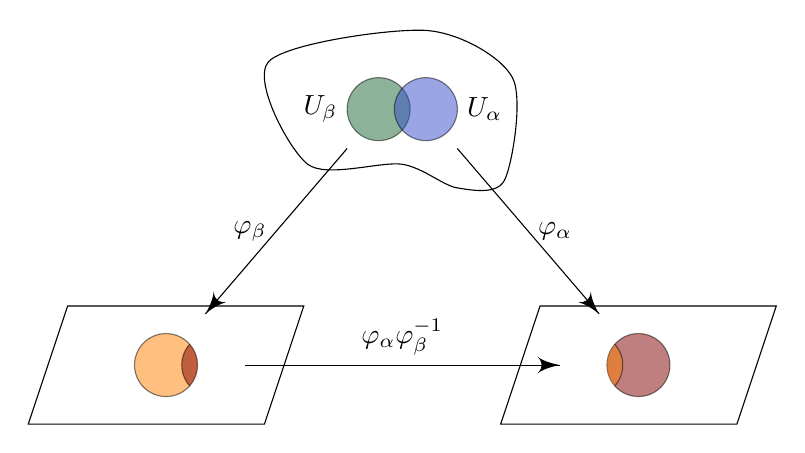
\begin{tikzpicture}
    \draw plot [smooth cycle] coordinates {(-1.2, -0.7) (0, -0.7) (0.7, -1) (1.3, -0.9) (1.4, 0.4) (0.3, 1) (-1.7, 0.6)};

    \draw (-0.3, 0) [fill=mgreen, opacity=0.5] circle [radius=0.4];
    \draw (0.3, 0) [fill=mblue, opacity=0.5] circle [radius=0.4];

    \node [left] at (-0.7, 0) {$U_\beta$};
    \node [right] at (0.7, 0) {$U_\alpha$};

    \begin{scope}[shift={(-4.75, -4)}]
      \draw (0, 0) -- (3, 0) -- (3.5, 1.5) -- (0.5, 1.5) -- cycle;

      \draw (1.75, 0.75) [fill=morange, opacity=0.5] circle [radius=0.4];
      \begin{scope}
        \clip (1.75, 0.75) circle [radius=0.4];
        \draw (2.35, 0.75) [fill=mred, opacity=0.5] circle [radius=0.4];
      \end{scope}
    \end{scope}

    \draw [->] (-0.7, -0.5) -- (-2.5, -2.6) node [pos=0.5, left] {$\varphi_\beta$};
    \draw [->] (0.7, -0.5) -- (2.5, -2.6) node [pos=0.5, right] {$\varphi_\alpha$};

    \begin{scope}[shift={(1.25, -4)}]
      \draw (0, 0) -- (3, 0) -- (3.5, 1.5) -- (0.5, 1.5) -- cycle;

      \draw (1.75, 0.75) [fill=mred, opacity=0.5] circle [radius=0.4];
      \begin{scope}
        \clip (1.75, 0.75) circle [radius=0.4];
        \draw (1.15, 0.75) [fill=morange, opacity=0.5] circle [radius=0.4];
      \end{scope}
    \end{scope}
    \draw [->] (-2, -3.25) -- (2, -3.25) node [pos=0.5, above] {$\varphi_\alpha \varphi_\beta^{-1}$};
  \end{tikzpicture}
\end{center}
$(U_\alpha, \varphi_\alpha)$  is called a \textbf{coordinate chart} and $\{(U_\alpha, \varphi_\alpha)\}_\alpha$ is called an \textbf{atlas}.  We can write
  \[
    \varphi_\alpha = (x^1, \cdots, x^n)
  \]
  where each $x_i: U_\alpha \to \R$. We call these the \textbf{local coordinates}. 

An important point of the definition of a smooth manifold is the following.  If $(U_\alpha, \varphi_\alpha)$ and $(U_\beta, \varphi_\beta)$ are charts in some atlas, and $f: M \to \R$, then $f \circ \varphi_\alpha^{-1}$ is smooth at $\varphi_\alpha(p)$ if and only if $f \circ \varphi_\beta^{-1}$ is smooth at $\varphi_\beta (p)$ for all $p \in U_\alpha \cap U_\beta$.


\begin{eg}
  Consider the sphere
  \[
    S^n = \{x=(x_0, \cdots, x_n)\in \R^{n+1}: \sum x_i^2 = 1\} .
  \]
  We define an atlas as follows. We define an open covering
  \[
    U^+ = S^n \backslash \{\textrm{south pole}\},\quad U^- = S^2 \backslash \{\textrm{north pole}\}~.
  \]
  where the south pole is $x_0=-1$ and the north pole is $x_0=1$, and continuous maps
  \begin{align*}
&    \varphi^+: U^+ \to \R^n; (x_0, \cdots, x_n) \mapsto \frac{1}{1+x_0}(x_1, \cdots, x_n)\\
  &  \varphi^-: U^- \to \R^n; (x_0, \cdots, x_n) \mapsto \frac{1}{1-x_0}(x_1, \cdots, x_n)\\
  \end{align*}
Then, their inverse maps are
  \begin{align*}
(\varphi^\pm)^{-1}:\R^n\to U^\pm;(y_1,\dots,y_n)\mapsto \frac{1}{1+|y|^2}(\pm(1-|y|^2),y_1,\dots,y_n)~.
  \end{align*}
The transformation map
$$
\varphi^+ \cdots(\varphi^-)^{-1}(y)=\frac{y}{|y|}    \quad \varphi^- \cdots(\varphi^+)^{-1}(y)=\frac{y}{|y|} 
$$
\end{eg}


Let $M$ and $N$  be smooth manifolds, and let $\{(U_\alpha, \varphi_\alpha)\}_\alpha$ and $\{(V_\beta, \psi_\beta)\}_\beta$ be their  atlas. We usually consider smooth maps between manifolds. 

\begin{defi}[Smooth map]\index{smooth map}
  A map $f: M \to N$ is \textbf{smooth} if, for a chart $(U_\alpha, \varphi_\alpha)$ of $p\in M$ and $(V_\beta, \psi_\beta)$ of $f(p)\in N$,  $ \psi_\beta \circ f \circ ( \varphi_\alpha)^{-1}: \varphi(U_\alpha \cap f^{-1} (V_\beta)) \to \xi(V_\beta )$ is smooth.


If it has smooth inverse, it is called \term{diffeomorphism}.

\end{defi}
\begin{center}
  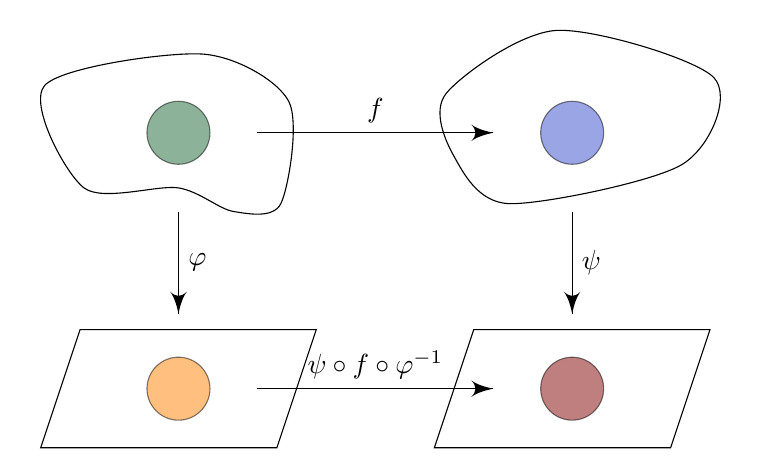
\begin{tikzpicture}
    \draw plot [smooth cycle] coordinates {(-1.2, -0.7) (0, -0.7) (0.7, -1) (1.3, -0.9) (1.4, 0.4) (0.3, 1) (-1.7, 0.6)};

    \draw [fill=mgreen, opacity=0.5] circle [radius=0.4];

    \begin{scope}[shift={(-1.75, -4)}]
      \draw (0, 0) -- (3, 0) -- (3.5, 1.5) -- (0.5, 1.5) -- cycle;

      \draw (1.75, 0.75) [fill=morange, opacity=0.5] circle [radius=0.4];
    \end{scope}

    \draw [->] (0, -1) -- +(0, -1.3) node [pos=0.5, right] {$\varphi$};
    \begin{scope}[shift={(5, 0)}]
      \draw plot [smooth cycle] coordinates {(1.4, -0.4) (-0.8, -0.9) (-1.5, -0.3) (-1.6, 0.5) (-0.2, 1.3) (1.8, 0.7)};

      \draw [fill=mblue, opacity=0.5] circle [radius=0.4];

      \begin{scope}[shift={(-1.75, -4)}]
        \draw (0, 0) -- (3, 0) -- (3.5, 1.5) -- (0.5, 1.5) -- cycle;

        \draw (1.75, 0.75) [fill=mred, opacity=0.5] circle [radius=0.4];
      \end{scope}

      \draw [->] (0, -1) -- +(0, -1.3) node [pos=0.5, right] {$\psi$};
    \end{scope}

    \draw [->] (1, 0) -- (4, 0) node [above, pos=0.5] {$f$};

    \draw [->] (1, -3.25) -- (4, -3.25) node [above, pos=0.5] {$\psi \circ f \circ \varphi^{-1}$};
  \end{tikzpicture}
\end{center}
Equivalently, $f$ is smooth at $p$ if $\xi \circ f \circ \varphi^{-1}$ is smooth at $\varphi(p)$ for \textbf{any} such charts $(U, \varphi)$ and $(V, \xi)$.

\section{Tangent space}




\begin{defi}[Tangent vector]\index{Tangent vector}
A \textbf{tangent vector} $X_p$ at $p\in M$ is a map $X_p:C^\infty(M)\to \R$, which is subject to 
\begin{description}
\item{linearity} $X_p(\alpha f+\beta g)=\alpha X_p(f)+\beta X_p(g)$,  for  $\alpha,\beta \in \R$
\item{Leibniz rule} $X_p(fg)=f(p)X_p(g)+X_p(f) g(p)$
\end{description}
\end{defi}
Namely, a  \textbf{tangent vector} $X_p$  behaves like a differential operator on $C^\infty(M)$. Then, the set of tangent vectors at $p$ become a vector space
$$
(X_p+Y_p)(f)=X_p(f)+Y_p(f) \qquad (\alpha X_p)(f)=\alpha (X_p(f))~,
$$
and we call it the \textbf{tangent space} $T_pM$ at $p\in M$.


\begin{figure}[h]\centering
\includegraphics[width=8cm]{Tangentialvektor}
\end{figure}



There is another way to think about tangent vectors. Let us consider a \term{curve}, which is a smooth map $\gamma:I \to M$ with $\gamma(0)=p$ where $I$ is a non-empty open interval. Two curves $\gamma_1,\gamma_2$ are \textbf{tangent} at $p$ if 
$$
\gamma_1(0)=p=\gamma_2(0)~, \qquad  \frac{d}{dt}\varphi(\gamma_1(t))\Big|_{t=0}= \frac{d}{dt}\varphi(\gamma_2(t))\Big|_{t=0}
$$
where $(U,\varphi)$ is a chart around $p$. We write  two tangent curves $\gamma_1\sim \gamma_2$, which forms an equivalence class.
\begin{figure}[h]\centering
\includegraphics[width=5cm]{tangent-curve}
\end{figure}
For ${}^\forall f\in C^\infty(M)$, We can then take the derivative of $f$ along $\gamma$ 
\[
  X_p(f) = \left.\frac{\d}{\d t}\right|_{t = 0} f(\gamma(t))~.
\]
It is easy to see that $X_p$ satisfies the definition of a tangent vector. So we can provide the definition of the tangent space at $p$ as
$$
T_pM=\{ \gamma:I\to M | \gamma(0)=p\}/\sim
$$
Given a local coordinate $\varphi=( x^1, \cdots, x^n)$, the tangent vector along a curve $\gamma$ can be written as
$$
X_p=\sum_{i=1}^n X_p^i\frac{\partial}{\partial x^i}\Big|_p   \quad \textrm{where} \quad X_p^i=\frac{d}{dt}x^i(\gamma(t))\Big|_{t=0}~.
$$
Therefore, $(\frac{\partial}{\partial x^1}\Big|_p,\cdots,\frac{\partial}{\partial x^n}\Big|_p)$ can be considered as a basis of $T_pM$.
Suppose we also have coordinates $y_1, \cdots, y_n$ near $p$ given by some other chart. Then, we can write 
\[
  \left.\frac{\partial}{\partial y_i}\right|_p = \sum_{j = 1}^n \frac{\partial x_j}{\partial y_i}(p)\left.\frac{\partial}{\partial x_j}\right|_p~,
\]
where $ \frac{\partial x_j}{\partial y_i}(p)$ is called \term{Jacobian} at $p$.


\section{Tangent bundles}
Let us consider a collection of tangent spaces over every point $p$ on $M$
\[
  TM = \bigcup_{p \in M} T_p M=\{(p,X_p)|p\in M ~, X_p\in T_pM\}~.
\]
into a manifold. There is then a natural map $\pi: TM \to M$ sending $X_p \in T_pM$ to $p$ for each $p \in M$, and this is smooth. 

We can consider $TM$ as a manifold of dimension $2 \dim M$, which is called the \textbf{tangent bundle} of $M$.
  Let $x^1, \cdots, x^n$ be coordinates on a chart $(U, \varphi)$. Then for any $p \in U$ and $X_p \in T_p M$, there are some $\alpha^1, \cdots, \alpha^n \in \R$ such that
  \[
    X^p = \sum_{i = 1}^n \alpha^i \left.\frac{\partial}{\partial x^i}\right|^{p}.
  \]
  This gives a bijection
  \begin{align*}
    \pi^{-1}(U) &\to \varphi(U) \times \R^n\\
    X^p &\mapsto (x^1(p), \cdots, x^n(p), \alpha^1, \cdots, \alpha^n),
  \end{align*}
  If $(V, \xi)$ is another chart on $M$ with coordinates $y^1, \cdots, y^n$, then
  \[
    \left.\frac{\partial}{\partial x^i}\right|^p = \sum_{j = 1}^n \frac{\partial y^j}{\partial x^i}(p) \left.\frac{\partial}{\partial y^j}\right|^p.
  \]
  So we have $\tilde{\xi} \circ \tilde{\varphi}^{-1}: \varphi(U \cap V) \times \R^n \to \xi(U \cap V) \times \R^n$ given by
  \[
    \tilde{\xi} \circ \tilde{\varphi}^{-1} (x^1, \cdots, x^n, \alpha^1, \cdots, \alpha^n) = \left(y^1, \cdots, y^n, \sum_{i = 1}^n \alpha^i \frac{\partial y^{1}}{\partial x^i}, \cdots, \sum_{i = 1}^n \alpha^i \frac{\partial y^n}{\partial x^i}\right),
  \]
  and is smooth (and in fact fiberwise linear).



\section{Vector fields}


A smooth map $X:M\to TM$ is called a \textbf{section} if $X\cdot \pi=id_M$. Since it is actually a smooth assignment $X:p \mapsto X(p)$, it is called a \term{vector field}. 

\begin{eg}
Let $S^n\subset \R^{n+1}$ be an $n$-sphere. We have a vector field 
$$
Y=\sum Y^i\frac{\partial}{\partial x^i}
$$
where 
$$
Y^i=\left\{ \begin{array}{ll} (-x^1,x^0,-x^3,x^2,\cdots,-x^{2k},x^{2k-1}) & n=2k+1\\ (-x^1,x^0,-x^3,x^2,\cdots,-x^{2k},x^{2k-1},0) & n=2k+2\end{array}\right.~.
$$
\end{eg}

\begin{figure}[h]\centering
\includegraphics[width=5cm]{vector-field}
\end{figure}

We write a set of vector fields by $\mathfrak{X}(M)=\Gamma(TM)$. In fact, a vector field $X\in \mathfrak{X}(M)$ is a map $C^\infty(M)\to C^\infty(M)$, which satisfies 
 \begin{align}\nonumber
& X(\alpha f+\beta g)=\alpha X(f)+\beta X(g),  \quad \textrm{for} \quad \alpha,\beta \in \R\cr
&X(fg)=fX(g)+X(f) g~.
\end{align}
Let $X, Y \in \mathfrak{X}(M)$, and $f \in C^\infty(M)$.   Then we have $X + Y, fX \in \mathfrak{X}(M)$. Therefore, $\mathfrak{X}(M)$ is a $C^\infty(M)$-module.



Note that the product of two vector fields $X,Y\in \mathfrak{X}(M)$ is not a vector field:
\begin{align*}
  XY(fg) &= X(Y(fg)) \\
  &= X(fY(g) + gY(f)) \\
  &= X(f) Y(g) + fXY(g) + X(g) Y(f) + g XY(f).
\end{align*}
 However, that $XY - YX$ is a vector field and we denote it as $[X, Y]$, called the \term{Lie bracket}. In fact, $\mathfrak{X}(M)$ with Lie bracket satisfies
  \begin{enumerate}
    \item $[\ph, \ph]$ is bilinear.
    \item $[\ph, \ph]$ is antisymmetric, i.e.\ $[X, Y] = -[Y, X]$.
    \item The \term{Jacobi identity} holds
      \[
        [X, [Y, Z]] + [Y, [Z, X]] + [Z, [X, Y]] = 0.
      \]
  \end{enumerate}



\section{Flows}
 An \term{integral curve} of $X \in \mathfrak{X}(M)$ is a smooth $\gamma: I \to M$ such that $I$ is an open interval in $\R$ and
  \[
    \dot{\gamma}(t) = X_{\gamma(t)}.
  \]

\begin{eg}
A vector field $X=\alpha \frac{\partial }{\partial x} +\beta  \frac{\partial }{\partial y}$ in $\R^2$. Then, the integral curve is a translation
$$
\gamma_t(x,y)=(x+t\alpha,y+t\beta)~.
$$  
\end{eg}



\begin{thm}[Existence of integral curves]
  Let $X \in \mathfrak{X}(M)$ and $p \in M$. Then there exists some open interval $I \subseteq \R$ with $0 \in I$ and an integral curve $\gamma: I \to M$ for $X$ with $\gamma(0) = p$.

  Moreover, if $\tilde{\gamma}: \tilde{I} \to M$ is another integral curve for $X$, and $\tilde{\gamma}(0) = p$, then $\tilde{\gamma} = \gamma$ on $I \cap \tilde{I}$.
\end{thm}

Let $M$ be a a compact manifold. A smooth map  
$$
\gamma:\R\times M \to M ; (t,p)\mapsto \gamma_t(p)
$$
is called \textbf{flow} (or one-parameter group of diffeomorphisms) generated by a vector $X$ if 
$$
\gamma_{t+s}(p)=\gamma_t(\gamma_s(p))~, \quad \frac{d\gamma_t(p)}{dt}=X_{\gamma_t(p)}~.
$$




\section{Orientation}
Suppose we have picked two ordered bases $(e_1, \cdots, e_n)$ and $(\tilde{e}_1, \cdots, \tilde{e}_n)$ of $T_pM$.  Then, we define an equivalence class  $(e_1, \cdots, e_n)\sim (\tilde{e}_1, \cdots, \tilde{e}_n)$ iff
\[
  e_i = \sum_j B_{ij} \tilde{e}_j \qquad  \det B > 0~.
\]
We call the two ordered bases have the \term{same orientation} if they are the same equivalence class. Therefore, for $p\in M$, we can assign an orientation $\mathcal{O}_p$. If we can give continuous assignment $p\mapsto \mathcal{O}_p$, then $M$ is called \term{orientable}.



A smooth manifold $M$ is orientable iff there exists an atlas  $\{(U_\alpha, \varphi_\alpha)\}_\alpha$ of $M$ such that the determinant of the Jacobian is positive on any $U_\alpha\cap  U_\beta$.


\begin{figure}[h]\centering
\includegraphics[width=4.5cm]{orientation-strip}
\caption{The M\"obius strip is not orientable.}
\end{figure}







\end{document}
